\documentclass[a4paper, 11pt]{article}

%%%%%% 导入包 %%%%%%
\usepackage{CJKutf8}
\usepackage{graphicx}
\usepackage[colorlinks,
            linkcolor=black,
            anchorcolor=black,
            citecolor=black,
            unicode]{hyperref}
\usepackage{xcolor}
\usepackage{cite}
\usepackage{indentfirst}
%%%%%% 设置字号 %%%%%%
\newcommand{\chuhao}{\fontsize{42pt}{\baselineskip}\selectfont}
\newcommand{\xiaochuhao}{\fontsize{36pt}{\baselineskip}\selectfont}
\newcommand{\yihao}{\fontsize{28pt}{\baselineskip}\selectfont}
\newcommand{\erhao}{\fontsize{21pt}{\baselineskip}\selectfont}
\newcommand{\xiaoerhao}{\fontsize{18pt}{\baselineskip}\selectfont}
\newcommand{\sanhao}{\fontsize{15.75pt}{\baselineskip}\selectfont}
\newcommand{\sihao}{\fontsize{14pt}{\baselineskip}\selectfont}
\newcommand{\xiaosihao}{\fontsize{12pt}{\baselineskip}\selectfont}
\newcommand{\wuhao}{\fontsize{10.5pt}{\baselineskip}\selectfont}
\newcommand{\xiaowuhao}{\fontsize{9pt}{\baselineskip}\selectfont}
\newcommand{\liuhao}{\fontsize{7.875pt}{\baselineskip}\selectfont}
\newcommand{\qihao}{\fontsize{5.25pt}{\baselineskip}\selectfont}

%%%% 设置 section 属性 %%%%
\makeatletter
\renewcommand\section{\@startsection{section}{1}{\z@}%
{-1.5ex \@plus -.5ex \@minus -.2ex}%
{.5ex \@plus .1ex}%
{\normalfont\sihao\CJKfamily{hei}}}
\makeatother

%%%% 设置 subsection 属性 %%%%
\makeatletter
\renewcommand\subsection{\@startsection{subsection}{1}{\z@}%
{-1.25ex \@plus -.5ex \@minus -.2ex}%
{.4ex \@plus .1ex}%
{\normalfont\xiaosihao\CJKfamily{hei}}}
\makeatother

%%%% 设置 subsubsection 属性 %%%%
\makeatletter
\renewcommand\subsubsection{\@startsection{subsubsection}{1}{\z@}%
{-1ex \@plus -.5ex \@minus -.2ex}%
{.3ex \@plus .1ex}%
{\normalfont\xiaosihao\CJKfamily{hei}}}
\makeatother

%%%% 段落首行缩进两个字 %%%%
\makeatletter
\let\@afterindentfalse\@afterindenttrue
\@afterindenttrue
\makeatother
\setlength{\parindent}{2em}  %中文缩进两个汉字位


%%%% 下面的命令重定义页面边距,使其符合中文刊物习惯 %%%%
\addtolength{\topmargin}{-54pt}
\setlength{\oddsidemargin}{0.63cm}  % 3.17cm - 1 inch
\setlength{\evensidemargin}{\oddsidemargin}
\setlength{\textwidth}{14.66cm}
\setlength{\textheight}{24.00cm}    % 24.62

%%%% 下面的命令设置行间距与段落间距 %%%%
\linespread{1.4}
% \setlength{\parskip}{1ex}
\setlength{\parskip}{0.5\baselineskip}

%%%% 正文开始 %%%%
\usepackage{ctex}
\begin{document}
\begin{CJK}{UTF8}{gbsn}

%%%% 定理类环境的定义 %%%%
\newtheorem{example}{例}             % 整体编号
\newtheorem{algorithm}{算法}
\newtheorem{theorem}{定理}[section]  % 按 section 编号
\newtheorem{definition}{定义}
\newtheorem{axiom}{公理}
\newtheorem{property}{性质}
\newtheorem{proposition}{命题}
\newtheorem{lemma}{引理}
\newtheorem{corollary}{推论}
\newtheorem{remark}{注解}
\newtheorem{condition}{条件}
\newtheorem{conclusion}{结论}
\newtheorem{assumption}{假设}

%%%% 重定义 %%%%
\renewcommand{\contentsname}{目录}  % 将Contents改为目录
\renewcommand{\abstractname}{摘要}  % 将Abstract改为摘要
\renewcommand{\refname}{参考文献}   % 将References改为参考文献
\renewcommand{\indexname}{索引}
\renewcommand{\figurename}{图}
\renewcommand{\tablename}{表}
\renewcommand{\appendixname}{附录}
\renewcommand{\algorithm}{算法}


%%%% 定义标题格式,包括title,author,affiliation,email等 %%%%
\title{基于光栅的裸眼3D技术\\调研报告第一部分}
\author{王子博,赵子瑞,鲁吴越,李嘉豪}
\date{2017年3月}


%%%% 以下部分是正文 %%%%
\maketitle

\tableofcontents
\newpage

\section{项目背景}

从二维的图像显示技术问世以来,如何让人享受到三维的视觉体验,就成了一个吸引人的问题。从生理上说,人的三维视觉体验主要有两个来源,一是双眼位置不同导致观看到的图像的细微差别,二是观看物体时眼球晶状体的聚焦位置。后者对于显示技术要求较高,因为固定的荧屏只能在一个特定的平面上成像,人眼观看时必然会聚焦在该平面上,而不可能聚焦在其他位置。因此,基于双目视差的三维显示技术发展较为成熟,是目前商业和市场应用的主流技术。接下来我们将简要介绍一下较为常见的若干历史技术。

\subsection{三维视觉体验的发展历史}

\subsubsection{双眼立体画}

\begin{figure}[h!]
  \centerline{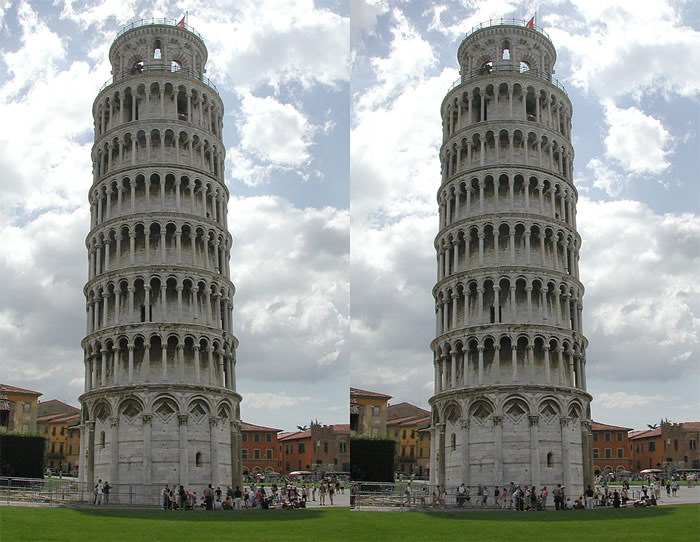
\includegraphics[width=8cm]{1.jpg}}
  \caption{一张双眼立体画}
\end{figure}

这是最为简单的一种技术,确切地说,它完全没有包含任何图像显示技术,仅仅是将双眼看到的图像分别印出。观看者需要想象在纸张背后无穷远处存在一个物体,并努力去观看该物体,以使得自己的两只眼睛直视前方,分别看到相应的图片(图\ref{fig2})。经过一些训练,观看者可以感受到两张图片合二为一,并产生看到了立体图形的体验。
\begin{figure}[h!]
  \centerline{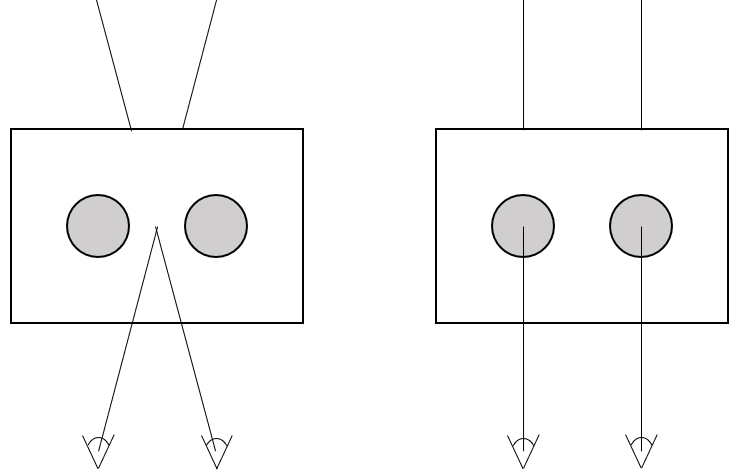
\includegraphics[width=8cm]{2.png}}
  \caption{双眼看纸面与双眼直视前方的区别}
  \label{fig2}
\end{figure}

这种立体画最大的一个局限就是人眼无法向两侧看,所以两张图片水平方向距离必须小于或等于瞳孔距离(约6厘米),无法制作出更大的图片。为了突破这一限制,以及让人观看起来更舒适,有类似于望远镜的工具出现,如图\ref{fig3},它能将距离较远的两张图通过光学器件送入人眼,方便观赏。
\begin{figure}[h!]
  \centerline{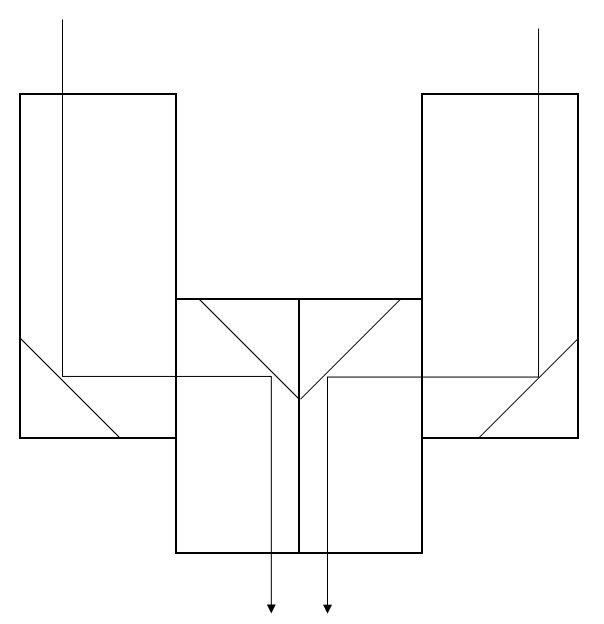
\includegraphics[width=3cm]{3.png}}
  \caption{立体视工具}
  \label{fig3}
\end{figure}

\subsubsection{红蓝眼镜}

\begin{figure}[h!]
  \centerline{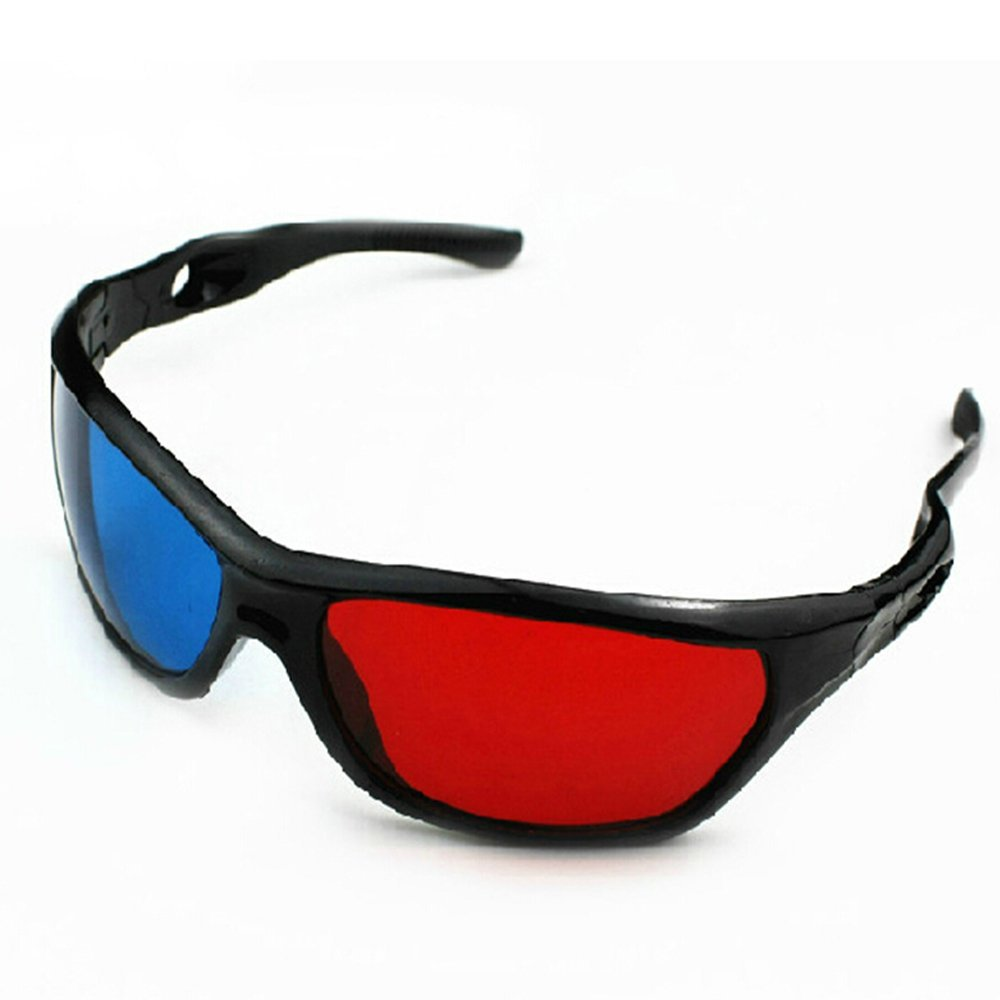
\includegraphics[width=8cm]{4.jpg}}
  \caption{一副红蓝眼镜}
\end{figure}

根据色彩原理,戴上红蓝眼镜后,双眼只能分别看到红色和蓝色分量,这两个分量的图像是独立的,因此可以为双眼提供不同的图像,组合出含有红色和蓝色分量的视觉感受,使人产生三维感。其缺点是双眼看到的颜色不同,会有强烈的冲突感,常常导致观看者感到画面红蓝闪烁,无法融入。

\subsubsection{偏振光眼镜}

根据光的偏振性原理,水平方向偏振的光无法穿过竖直方向的偏振膜,竖直方向偏振的光亦无法穿过水平方向的偏振膜。因此,可以制成一种眼镜,其两只镜片覆盖了互相垂直的偏振膜,而屏幕上同时以两种偏振方向的光分别呈现左右眼的画面,通过眼镜就可以感受到三维视觉。这种技术的缺点主要在于需要特殊的显示装置,而且观众观看时不可以将头倾斜,否则每只眼睛都会看到一些另一只眼睛应当看到的图像,体验并不舒适。

\subsubsection{电子快门眼镜}

\begin{figure}[h!]
  \centerline{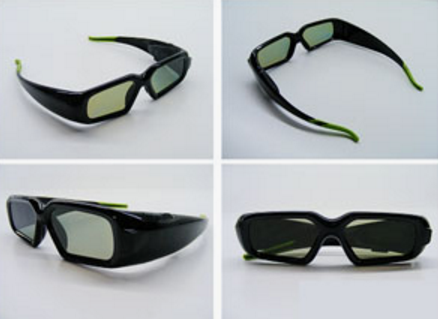
\includegraphics[width=8cm]{5.png}}
  \caption{一副电子快门眼镜}
\end{figure}

电子快门型3D显示技术也称为主动式3D(Active Shutter 3D),

这种眼镜的两只镜片受电信号控制,可以快速地在透光和不透光状态间转换。此技术在相当长的时期内被用于播放3D电影。播放时,左右眼应当看到的画面会以较高频率轮流在银幕上展示,另有一个红外线信号指示出当前正在显示的内容应当由左眼还是右眼看到。眼镜上的红外接收装置会根据这个信号来遮挡住一只眼睛,只让另一只眼睛看到画面。由于交替频率高,根据人眼的视觉暂留效应,观众不会感觉到画面交替,而是会感觉到两只眼睛看到了不同的视频内容,因此产生3D体验。

\subsection{裸眼3D技术的优势}

从以上总结可以看出,历史上的三维视觉体验技术,常常需要观看者做出特殊的动作,或者佩戴特殊的设备,这阻碍了三维视觉体验技术的普及。所谓“裸眼3D技术”,就是指观看者不需要佩戴任何设备,直接注视屏幕,即可感受到三维效果的技术。

\section{技术细节}

\subsection{选择光栅的原因}

目前能让裸眼两只眼睛看到不同画面的技术主要有全息摄影, 光栅遮挡法, 光栅分光法和指向性光源技术. 我们小组希望找到一种简单廉价的选择, 只在屏幕上覆盖一层膜, 无须使用特殊显示器, 即可让观看者体验到三维视觉. 因此, 我们尝试了光栅遮挡法(图\ref{fig6})和光栅分光法(图\ref{fig7}). 其中前者的原理是在屏幕前设置一个黑色线条和透明部分不断交替的光栅层,从左眼的视角看,这些黑色线条恰遮挡住所有偶数列的像素,而从右眼的视角看,这些黑色线条恰遮挡住所有奇数列的像素.这种技术不仅会导致屏幕亮度损失一半,而且对于用户头部移动过于敏感.通过简单的计算不难发现,用户只要水平移动头部3厘米,左眼和右眼所看到的画面就会恰好颠倒,三维效果完全被破坏.我们没有选择这种技术,而选择了光栅分光法.其原理是使用一系列柱状透镜改变光路,使得只有特定的像素能被左眼和右眼分别看到.这种技术比光栅遮挡法难研究,但可以产生非常好的观看效果.图\ref{fig8}和图\ref{fig9}分别是从两个角度拍摄的使用光栅分光法制成的三维效果卡片,这种卡片非常廉价且观赏效果令人叹服.
\begin{figure}[h!]
  \centerline{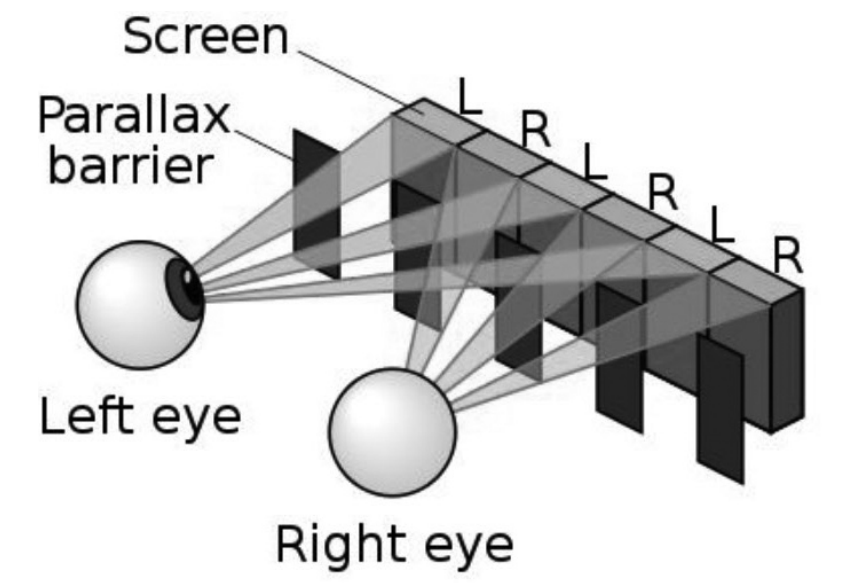
\includegraphics[width=\linewidth]{6.png}}
  \caption{光栅遮挡法}
  \label{fig6}
\end{figure}
\begin{figure}[h!]
  \centerline{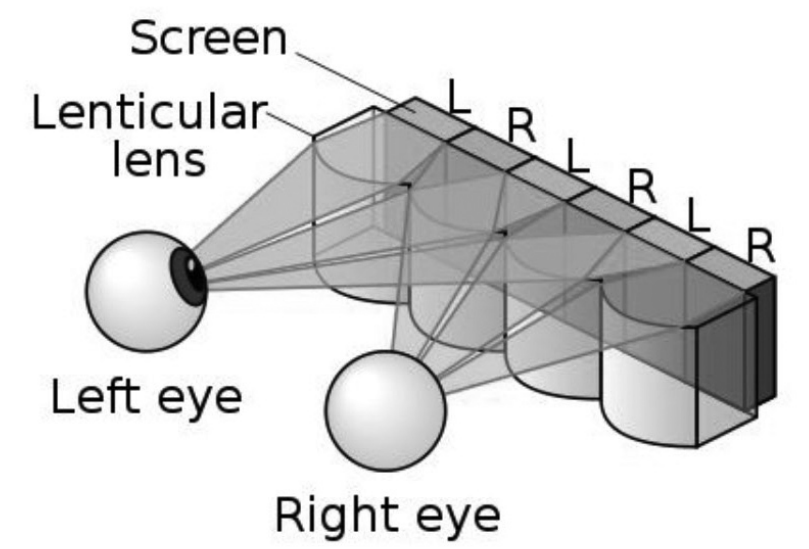
\includegraphics[width=\linewidth]{7.png}}
  \caption{光栅分光法}
  \label{fig7}
\end{figure}

\begin{figure}[h!]
  \centerline{\includegraphics[width=\linewidth]{IMG_20170319_213556.jpg}}
  \caption{一个角度拍摄的卡片}
  \label{fig8}
\end{figure}
\begin{figure}[h!]
  \centerline{\includegraphics[width=\linewidth]{IMG_20170319_213602.jpg}}
  \caption{另一个角度拍摄的卡片}
  \label{fig9}
\end{figure}

\begin{figure}[h!]
  \centerline{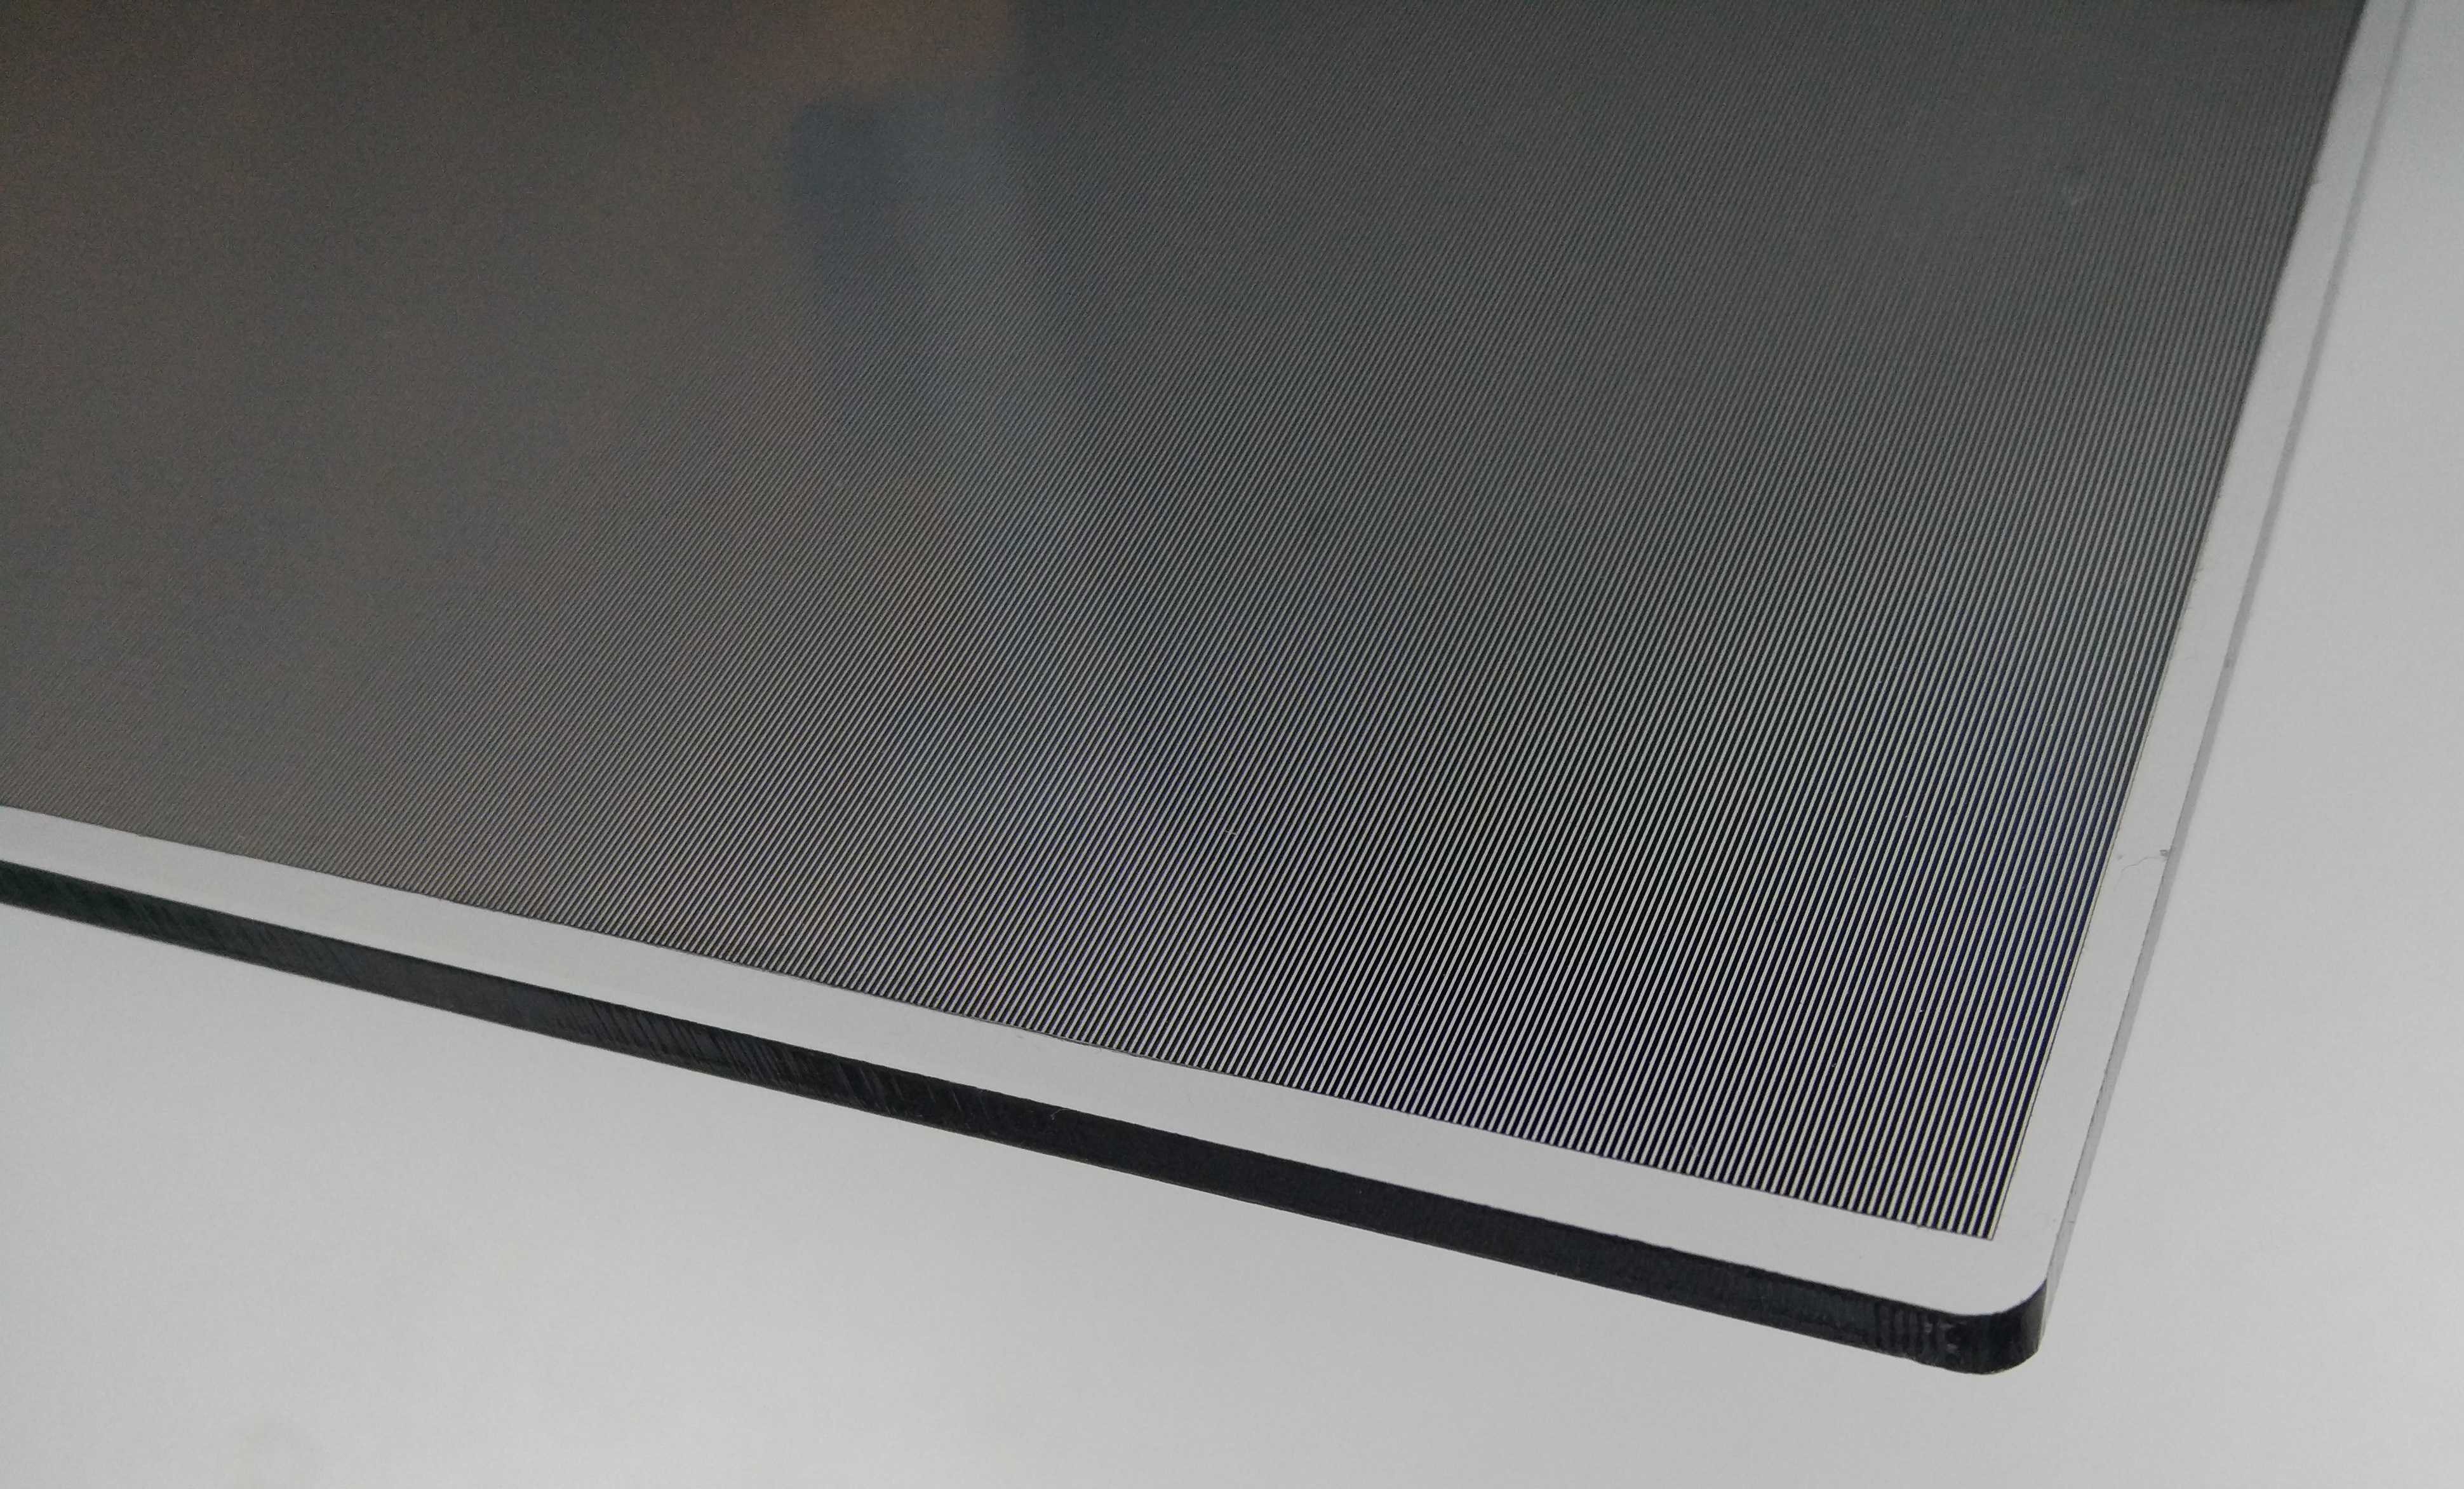
\includegraphics[width=\linewidth]{IMG_20170319_213725.jpg}}
  \caption{购买的遮挡型光栅之一}
\end{figure}
\begin{figure}[h!]
  \centerline{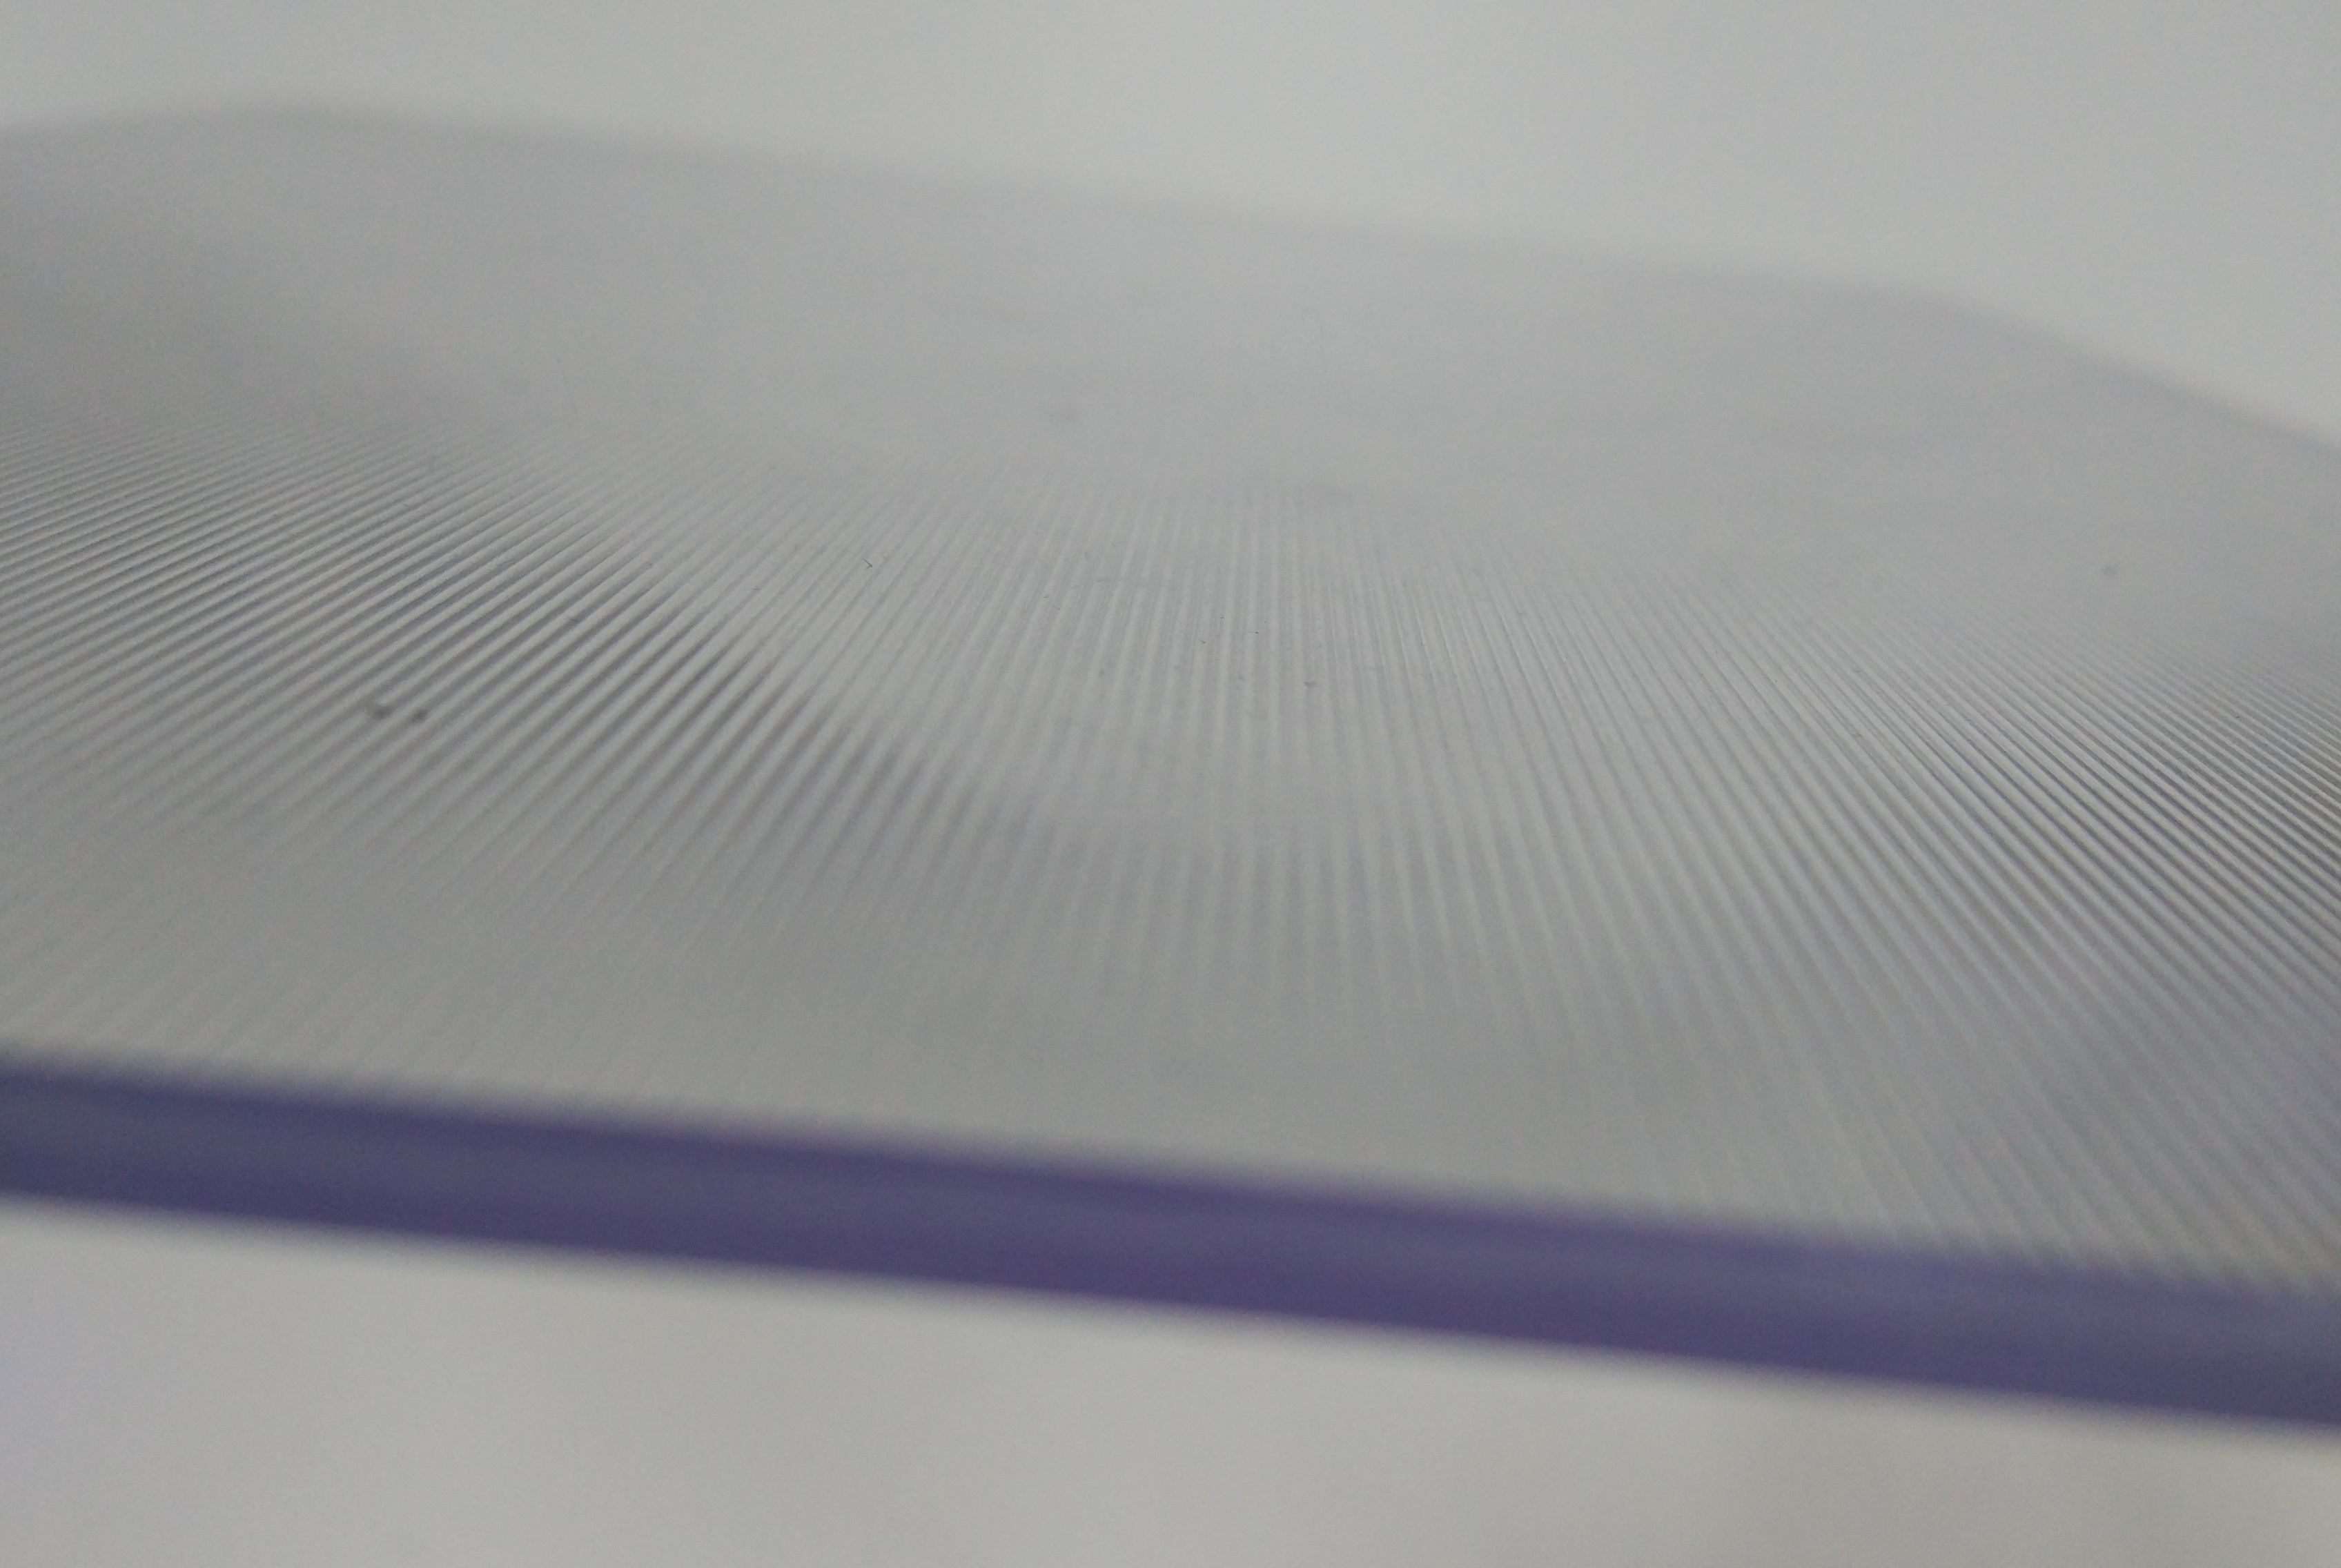
\includegraphics[width=\linewidth]{IMG_20170319_213819.jpg}}
  \caption{购买的分光型光栅之一}
\end{figure}

\subsection{主要难点}

这个项目有两大技术难点:

一是需要研究光栅的光学特性,弄清楚其对于显示屏发出的光的影响,了解观看者看到的图案的成因.尤其是研究当光栅放置得不完美时,例如略微倾斜或未与像素对齐时的情形,为使用软件手段弥补这类错误打下基础.

二是开发一个软件工具,它需要带有易用的检测工具,能够通过显示测试图样并接受用户反馈来检测用户实际摆放光栅的线密度,角度和位置.收集这些信息后,它可以接受视频源,游戏引擎输出或静态图像,将其渲染为合适的图案,使用户看到高质量的三维效果.

目前项目尚处在可行性研究阶段,因此我们主要的工作是在研究光学性质.之后将会更多地攻克第二个技术难点.以下分别介绍目前在两个方向所做出的努力.

\subsection{光学性质研究}

这个项目需要进行大量光学方面的研究, 以探索光栅对于发光源的分光作用, 模拟用户看到的画面. 为此,我们自行开发了一个光学模拟平台-Grating Simulation Platform (GSP). 该平台由Python编写, 前端界面由PyGame提供, 允许用户在工作区放置若干光源, 光栅, 透镜. 并且能够追踪光线, 计算实际折射情形。本小节的图片皆由GSP模拟平台产生。

目前所有的3D产品的基本思想都是让人的两只眼睛可以分别接收到不同的图像, 而我们采用的圆柱形3D光栅可以在很大程度上达到这样的目的. 圆柱形3D光栅的横截面如图\ref{fig:226}所示. 这种光栅的截面由一系列小的圆柱形的棱构成. 图\ref{fig:227}给出了我们描述棱的参数的一些符号约定.
\begin{figure}[h!]
  \centerline{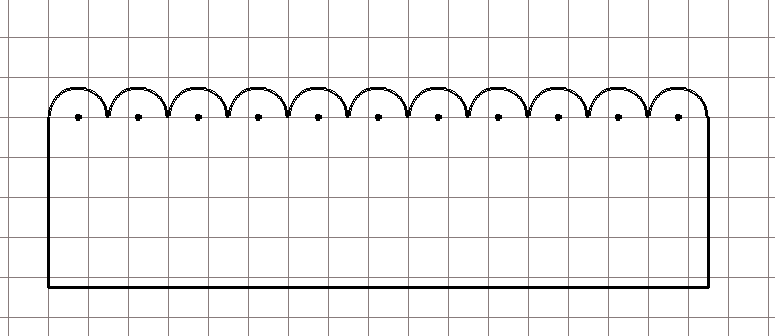
\includegraphics[width=\linewidth]{226.png}}
  \caption{圆柱形3D光栅的横截面示意图}
  \label{fig:226}
\end{figure}
\begin{figure}[h!]
  \centerline{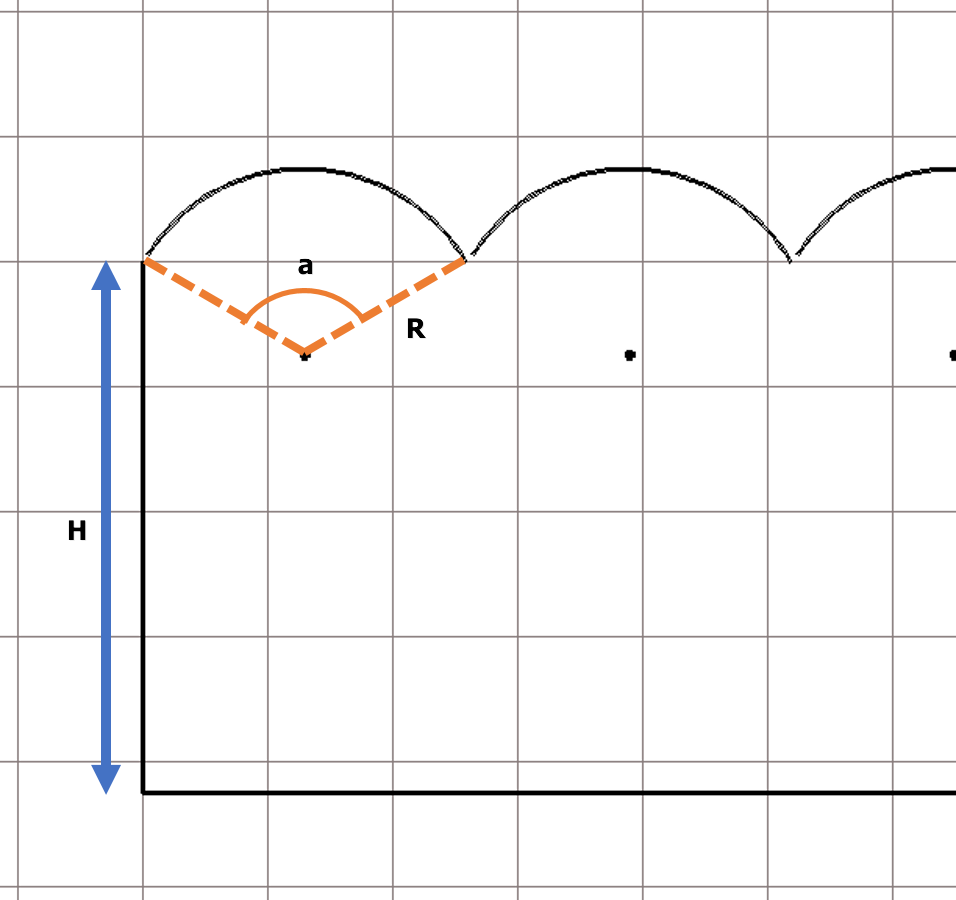
\includegraphics[width=8cm]{227.png}}
  \caption{描述圆柱形的参数的符号}
  \label{fig:227}
\end{figure}

从横截面示意图可以看出光栅上一系列的小圆柱体构成一系列的透镜组, 位于光栅后面的像素点会在不同的方向成像, 这样一来, 对于一个像素点, 只有在一些特定的角度才能够被看到. 这样就拥有了将两只眼睛需要看到的景象分开的能力. 对于单个像素点对, 在这样的棱镜组中成像的结果如图\ref{fig:217}所示:
\begin{figure}[h!]
  \centerline{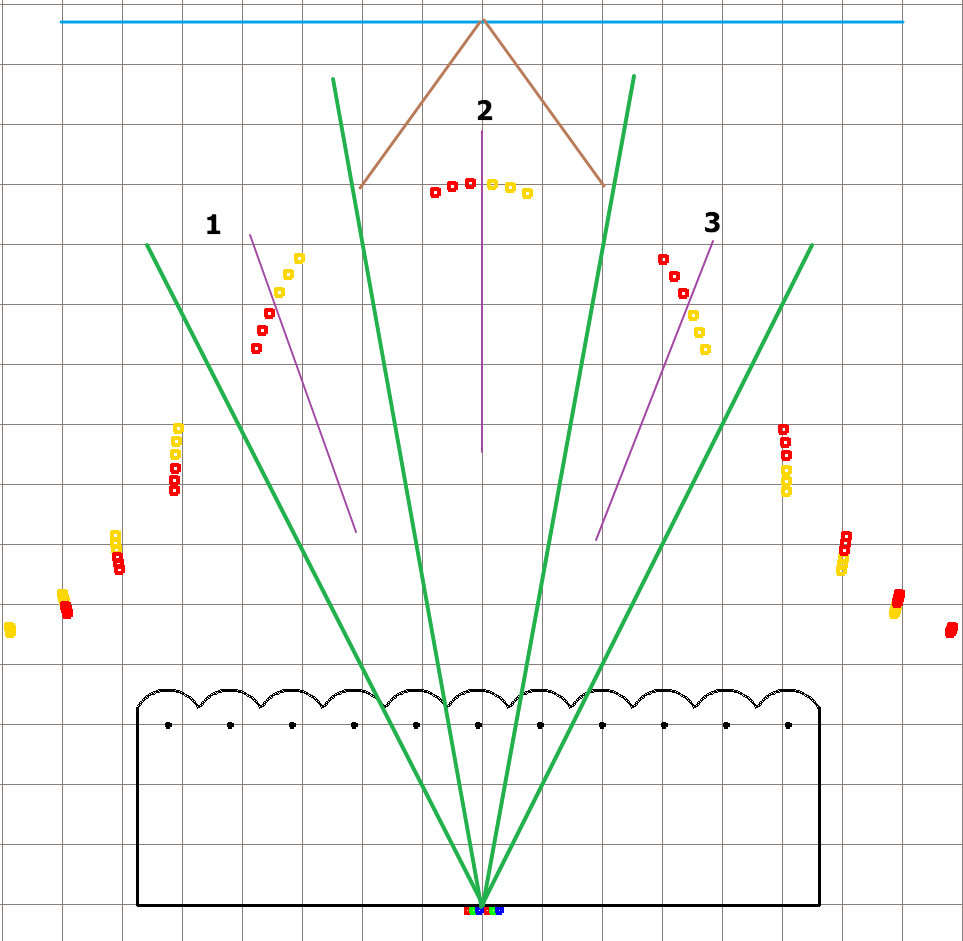
\includegraphics[width=10cm]{217.png}}
  \caption{单个像素点对的成像情况, 其中红色和黄色的点代表两个像素经过光栅之后成的像, 蓝线是用户习惯的观察距离, 棕色的线是用户观察图片时视野的张角.}
  \label{fig:217}
\end{figure}

图\ref{fig:217}中有两个像素点, 他们成的像分别使用红色和黄色的像点表示. 可以很清晰地看出来, 总共有3个主要的观察角度可以看到这一对点的像, 人眼在这些区域可以保证两只眼睛看到不同的像素点. 所以我们可以将所有的像素点分为两类. 一类负责显示左眼看到的图像, 另一类负责显示右眼看到的图像. 于是我们可以考虑使用若干个连续的像素去显示一只眼睛所看到的景象, 这两种像素段交替出现, 我们将这种像素段称为一个单元. 比如图\ref{fig:223}就是这两类像素每3个为一组交替出现的情形.
\begin{figure}[h!]
  \centerline{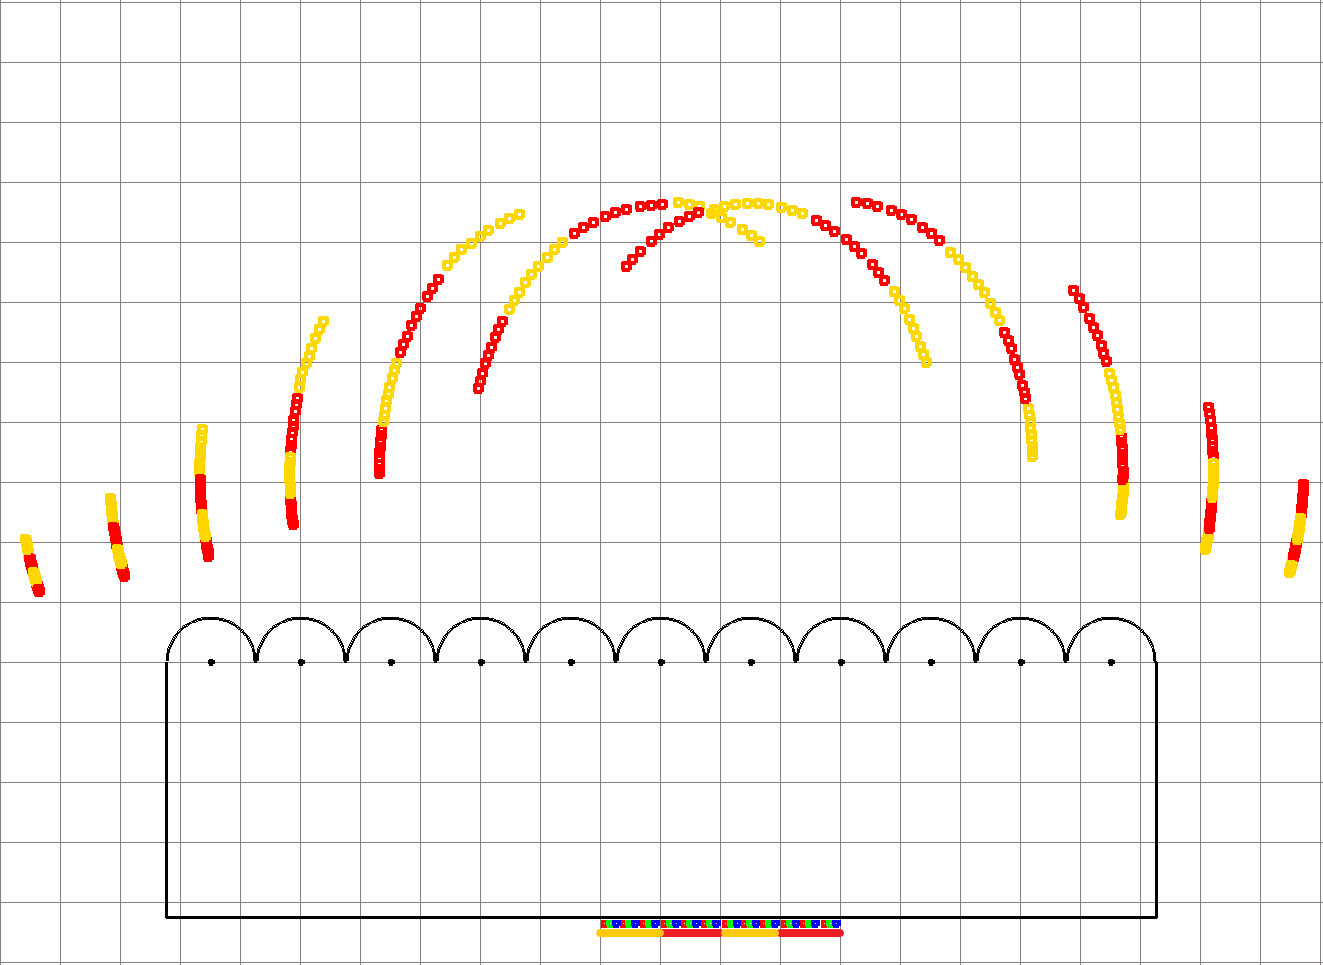
\includegraphics[width=8cm]{223.png}}
  \caption{两类像素交替出现的周期是3 的情形}
  \label{fig:223}
\end{figure}

同一种颜色的区域对应的像素是一只眼睛看到的结果. 结果可以看出, 我们对于一对单元, 确实可以在不同的区域显示出不同的眼睛看到的图像. 当我们增加像素点的个数去接近现实情况时. 模拟的结果如图\ref{fig:225}所示.
\begin{figure}[h!]
  \centerline{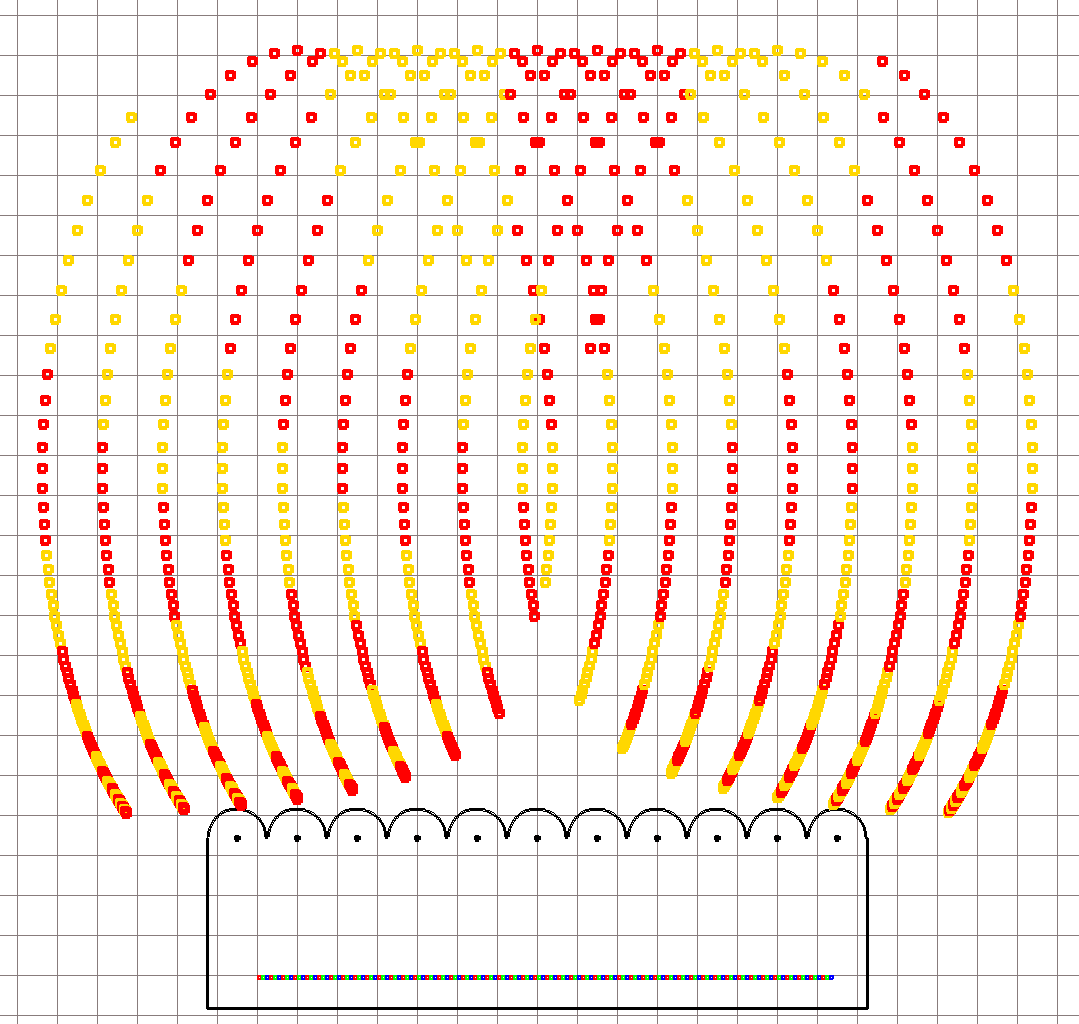
\includegraphics[width=8cm]{225.png}}
  \caption{大面积像素点的行为}
  \label{fig:225}
\end{figure}

这张图里, 总共有48个像素点成像, 共8个单元. 我们可以很明显看出来在不同的观察扇区能够看到不同的图像. 但是值得注意的是, 人眼观察事物是有一个张角的, 所以单个扇区必须对人眼张角要足够大, 否则一只眼睛就可以看到一个以上的扇区了, 导致3D效果缺失. 所以像素距离里圆柱中心的距离非常重要, 因为像素距离圆柱中心的距离决定了成像的扇区的大小, 比如图\ref{fig:228}的是像素里光栅过于远的情况. 由于扇区的间隔过小. 导致3D 效果消失. 同时, 如果像素过于靠近圆柱中心也会失败, 因为成像点远远超出正常人的使用范围,如图\ref{fig:229}. 所以光栅的厚度非常重要. 除此之外, 圆柱的夹角a和圆柱的半径R也会因为影响圆柱的焦距而导致像点过近或者过远的情况出现. 从而导致3D 效果失真. 图\ref{fig:231} 和图\ref{fig:232}说明了这一现象.
\begin{figure}[h!]
  \centerline{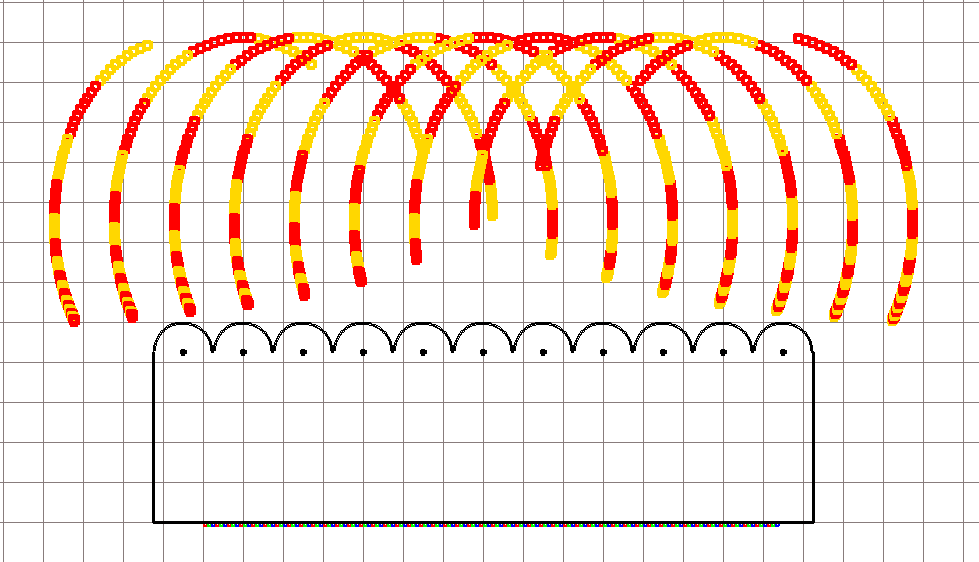
\includegraphics[width=8cm]{228.png}}
  \caption{大面积像素点的行为}
  \label{fig:228}
\end{figure}

\begin{figure}[h!]
  \centerline{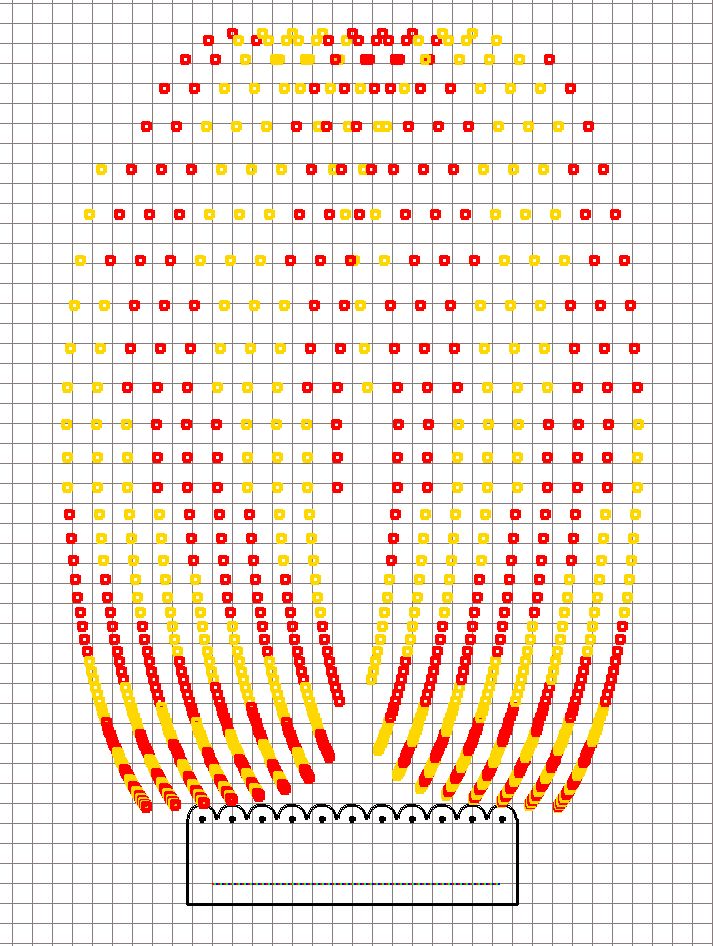
\includegraphics[width=8cm]{229.png}}
  \caption{像素过于靠近圆柱中心时两种图像重叠}
  \label{fig:229}
\end{figure}

除此之外我们还可以放置更多种类的像素, 比如图\ref{fig:230}中有3种像素. 所以我们可以放上在3个角度观察到的图像. 这样3D效果会被进一步增强. 因为人们能够感觉到可以从不同的角度去观察物体的感觉. 这些模拟已经基本展现出了使用光栅技术达到裸眼3D的原理和可行性.

\begin{figure}[h!]
  \centerline{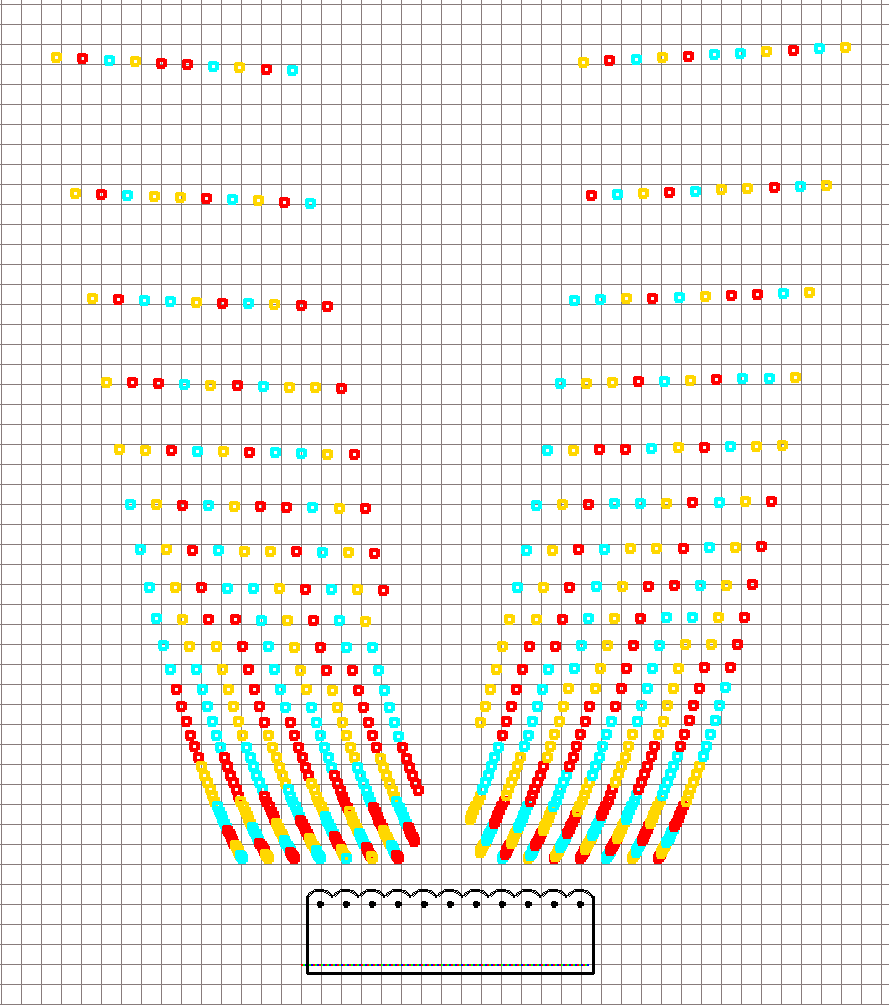
\includegraphics[height=14cm]{231.png}}
  \caption{当圆柱形的张角a减小时圆柱的焦距变大, 不合适的张角会导致3D效果失真}
  \label{fig:231}
\end{figure}

\begin{figure}[h!]
  \centerline{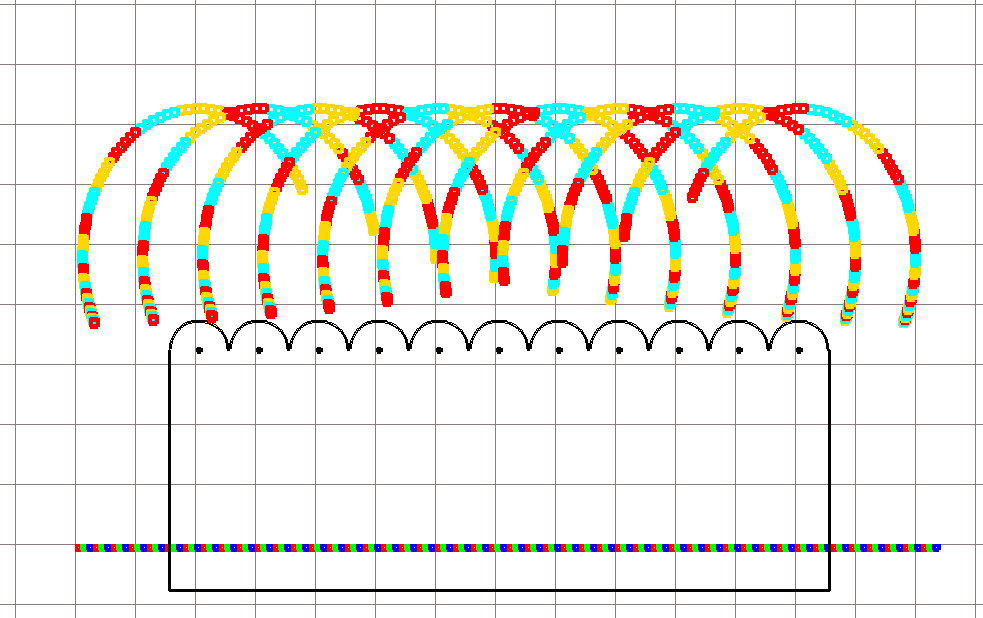
\includegraphics[width=10cm]{232.png}}
  \caption{当圆柱半径减小时会导致圆柱焦距变小, 不合适的间隔会导致3D效果失真}
  \label{fig:232}
\end{figure}

\begin{figure}[h!]
  \centerline{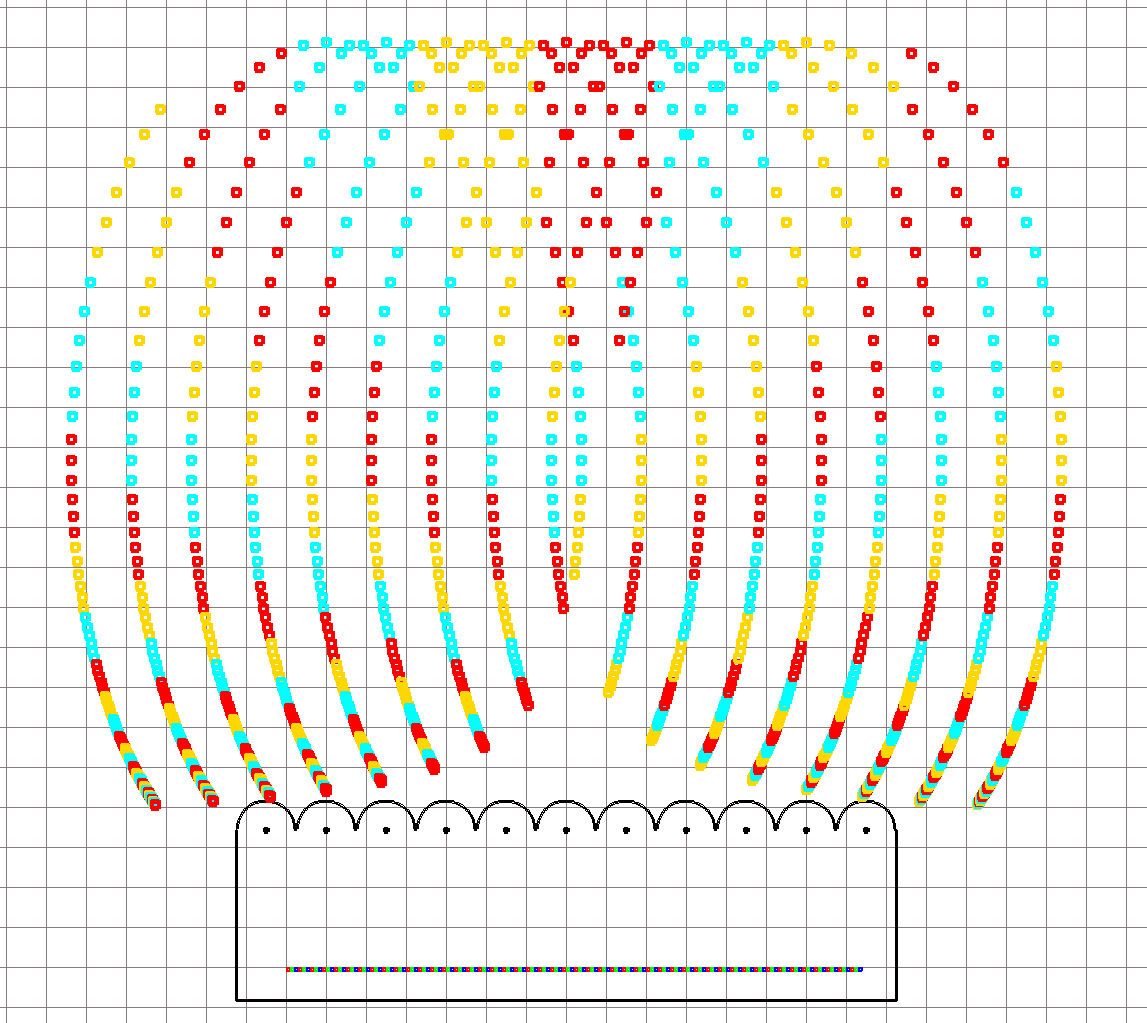
\includegraphics[height=8cm]{230.png}}
  \caption{3种像素的效果}
  \label{fig:230}
\end{figure}

除此之外我们还可以放置更多种类的像素, 比如图\ref{fig:230}中有3种像素. 所以我们可以放上在3个角度观察到的图像. 这样3D效果会被进一步增强. 因为人们能够感觉到可以从不同的角度去观察物体的感觉. 着一些模拟已经基本展现出了使用光栅技术达到裸眼3D的原理和可行性.

\subsection{测试平台搭建}

在软件开发方面,为了对买到的实际光栅进行测试,我们开发了一系列光栅研究工具,并用它们做了一些前期试验.

我们主要使用的测试平台是由Python调用pygame库在屏幕上绘图,通过电脑上运行的VNC服务器

\subsection{可行性测试}

\section{前沿工作}

\subsection{指向光源技术}
指向光源(Directional Backlight)是一种新型的3D技术, 其搭配两组LED,配合快速反应的LCD面板和驱动方法,让3D 内容以排序方式进入观看者的左右眼互换影像产生视差,进而让人眼感受到3D三维效果. 其基本原理示意图如图\ref{fig:233}所示.目前对指向光源3D 技术投入较大精力的主要是3M公司. 前不久,3M 公司刚刚展示了其研发成功的3D 光学膜,该产品的面试实现了无需佩戴 3D 眼镜,就可以在手机,游戏机及其他手持设备中显示真正的三维立体影像,极大地增强了基于移动设备的交流和互动。但是这项技术目前还在开发当中, 并不成熟.

\begin{figure}[h!]
  \centerline{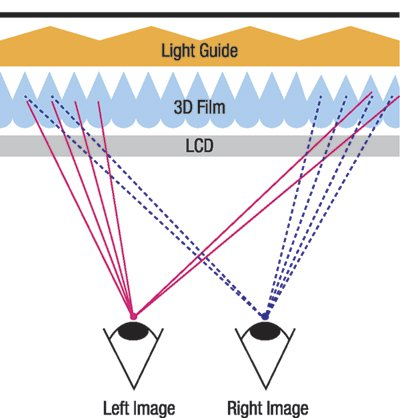
\includegraphics[width=10cm]{233.jpg}}
  \caption{指向光源技术的原理示意图}
  \label{fig:233}
\end{figure}

\subsection{裸眼3D的实际产品}
在2010年, 任天堂推出了一款使用裸眼3D屏幕的游戏机-3DS. 裸眼3D技术第一次走进了消费者的视野中. 但是这一款产品有很多的缺点. 比如其分辨率非常低, 上屏幕分辨率只有800×240像素, 下屏幕分辨率只有320×240像素. 大小都只有4~5英寸. 实际使用的效果并不会很好. 并且其售价也非常高.

\begin{figure}[h!]
  \centerline{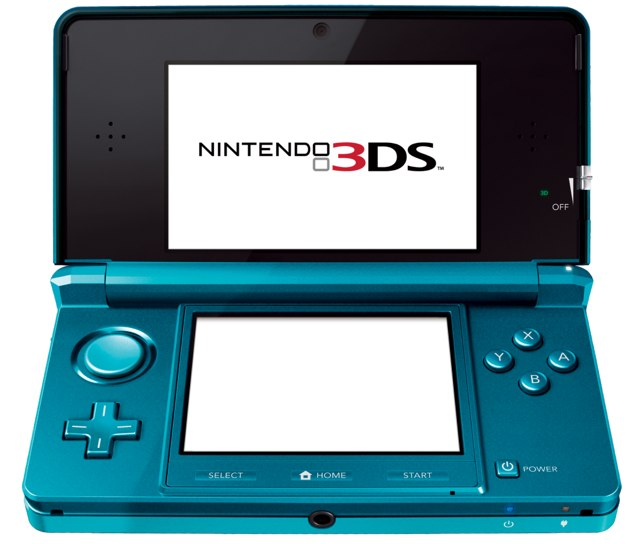
\includegraphics[width=10cm]{234.jpg}}
  \caption{任天堂的3DS游戏机}
  \label{fig:234}
\end{figure}

\subsection{与前沿工作的对比}
目前这些前沿的技术一般都有一下一些问题. 比如通用性很差, 必须要使用一些特定的硬件才能够使用, 比如3DS. 并且这一类产品的价格也都相对很高. 但是我们的目标是降低裸眼3D对硬件的依赖. 将优化主要留给软件. 这样即可以提高通用性, 也可以降低成本.

\end{CJK}
\end{document}
